\documentclass{beamer}
\usepackage{beamerthemesplit}
\usepackage{wrapfig}
\usetheme{SPbGU}
\usepackage{pdfpages}
\usepackage{amsmath}
\usepackage{cmap} 
\usepackage[T2A]{fontenc} 
\usepackage[utf8]{inputenc}
\usepackage[english,russian]{babel}
\usepackage{indentfirst}
\usepackage{amsmath}
\usepackage{tikz}
\usepackage{multirow}
\usepackage[noend]{algpseudocode}
\usepackage{algorithm}
\usepackage{algorithmicx}
\usetikzlibrary{shapes,arrows}
\usepackage{fancyvrb}
\usepackage{tikz}
\usepackage{pgfplots}
\usetikzlibrary{calc}
\usetikzlibrary{shapes,arrows}
\usetikzlibrary{arrows,automata}
\usetikzlibrary{positioning}
\usepackage[labelformat=empty]{caption}
\usepackage[labelformat=empty]{subcaption}
\beamertemplatenavigationsymbolsempty
\usepackage{multirow}
\usepackage{verbatim}
\usepackage{array}
\usepackage{graphicx}
\usepackage{multirow} 
\usepackage{fancyvrb}
\usepackage[misc,geometry]{ifsym} 
\newcolumntype{P}[1]{>{\centering\arraybackslash}p{#1}}


\newcommand{\tikzmark}[1]{\tikz[overlay,remember picture] \node (#1) {};}
\def\Put(#1,#2)#3{\leavevmode\makebox(0,0){\put(#1,#2){#3}}}

\newcommand{\ltz}{$< 1$}
\tikzset{
    state/.style={
           rectangle,
           rounded corners,
           draw=black, very thick,
           minimum height=2em,
           inner sep=4pt,
           text centered,
           },
}

\newtheorem{rutheorem}{Теорема}
\newtheorem{task}{All-paths CFPQ problem and reachability CFPQ problem }
\newtheorem{ruproof}{Доказательство}
\newtheorem{rudefinition}{Определение}
\newtheorem{rulemma}{Лемма}


\title[]{Implementation and experimental study of GLL algorithm with Neo4j graph database}
% То, что в квадратных скобках, отображается в левом нижнем углу. 
\institute[SPbU]{
St Petersburg State University}

% То, что в квадратных скобках, отображается в левом нижнем углу.
\author[Pogozhelskaya Vlada]{Pogozhelskaya Vlada Vladimirovna, 18.Б11-мм \\
  % У научного руководителя должна быть указана научная степень
  \and  
    {\bfseries Supervisor:} Ph.D. of Physico-mathematical Sciences, Associate Professor of the Department of Informatics of St Petersburg State University S.V. Grigoriev \\ 
  % Для курсовой не обязателен. Должна быть указана должность или ученая степень
}

\date{April 30, 2022}

\definecolor{orange}{RGB}{179,36,31}

\begin{document}
{
% Лого университета или организации, отображается в шапке титульного листа
\begin{frame}
  \begin{center}
  {
\includegraphics[width=1.2cm]{pics/SPbGU_Logo.png}}
  \end{center}
  \titlepage
\end{frame}
}
\begin{frame}[fragile]
  \transwipe[direction=90]
  \frametitle{Introduction}
  \begin{itemize}
      \item Graph data model
      \begin{itemize}
        \item Basic entities --- graph vertices
        \item Relationships between entities are graph edges
      \end{itemize}
    \item Graph databases
\begin{itemize}
    \item The most popular is Neo4j
    \item Only regular queries are partially supported
\end{itemize} 
\item Context-free constraints
\begin{itemize}
    \item Strictly more expressive than the regular one
    \item Widely used in bioinformatics, RDF file analysis, static code analysis
\end{itemize}
\end{itemize}
\end{frame}

\begin{frame}[fragile]
  \transwipe[direction=90]
  \frametitle{Context-free path querying problems}
   \begin{task}
  Let be:
     \begin{itemize}
    \item Context-free grammar $\mathbb{G}  = \langle N, \Sigma, P, S \rangle$
     \item Directed graph $ \mathbb{D} = \langle V, E, T \rangle$
     \item Set of start vertices $V_S \subseteq V$  and set of final vertices \mbox{$V_F \subseteq V$}
\end{itemize} 
\textbf{All-paths problem}:
\begin{itemize}
    \item Find all paths $\pi = (e_1, \cdots, e_{n - 1}, e_n), ~ e_k = (v_{k - 1}, t_k, v_k)$ in graph $ \mathbb{D}$, such as $l(\pi) = t_1t_2 \cdots t_n \in L(\mathbb{G})$ and $v_0 \in V_S, ~v_n \in V_F$
\end{itemize}
\textbf{Reachability problem}:
\begin{itemize}
    \item Find all pairs $\{(v_0, v_n ) ~|~ exists~a~path ~\pi = (e_1, \cdots, e_{n - 1}, e_n), ~ e_k = (v_{k - 1}, t_k, v_k)~ in ~\mathbb{D}, ~v_0 \in V_S, ~v_n \in V_F, ~l(\pi) = t_1t_2 \cdots t_n \in L(\mathbb{G}) \}$
\end{itemize}
 \end{task}
\end{frame}

\begin{frame}[fragile]
  \transwipe[direction=90]
  \frametitle{Motivation}
  \begin{itemize}
        \item The problem of poor performance of CFPQ algorithms was formulated by Jochem Kuijpers as a result of an attempt to extend Neo4j\footnote{An Experimental Study of Context-Free Path Query Evaluation Methods / Jochem Kuijpers, George Fletcher, Nikolay Yakovets, Tobias Lindaaker / SSDBM ’19}
      \item Later, the matrix-based CFPQ algorithm showed high performance on real-world data
  \end{itemize}
\end{frame}

\begin{frame}
  \transwipe[direction=90]
  \frametitle{Goal and tasks}
  \textbf{The aim} of this work is to improve existing CFPQ
algorithm for the Neo4j graph database\footnote{Algoruthm implementation: \url{https://github.com/JetBrains-Research/GLL4Graph/tree/8be59e6b314a1bfa646b119f751b3f28ad34ac64}} and evaluate it
  
  \textbf{Tasks}:
  \begin{itemize}
  \item To make initial experiments and analysis of existing algorithm to identify performance problems
    \item To refactor the code of the current implementation of the GLL-based CFPQ algorithm in order to identifying and eliminate performance problems of the current implementation of the algorithm
    \item To provide an ability to obtain information about both reachability CFPQ problem in a graph and all paths CFPQ problem
    \item To evaluate the resulting algorithm on real-world graphs and to compare it with an existing one
\end{itemize}
\end{frame}

\begin{frame}
  \transwipe[direction=90]
  \frametitle{Overview}
  \textbf{Generalized LL algorithm (GLL)}
\begin{itemize}
    \item Supports the entire class of context-free languages
    \item To reconstruct the paths, the Shared Packed Parse Forest (SPPF) is used
\end{itemize}
\textbf{Proposed solution}\\
  \begin{itemize}
    \item Based on GLL algorithm implementation in Iguana\footnote{ Repository of Iguana project: \url{https://github.com/iguana-parser/iguana}} project made at CWI Amsterdam in 2016
    \item Neo4j graph database is used as a graph storage
    \item The solution was integrated with Neo4j using Native Java API
  \end{itemize}
  \end{frame}
  
  \begin{frame}
  \transwipe[direction=90]
 \frametitle{Initial experiments}
An unexpected deterioration in the behavior of the resulting solution was revealed in the multiple-source scenario
    
\begin{figure}[H]
\centering
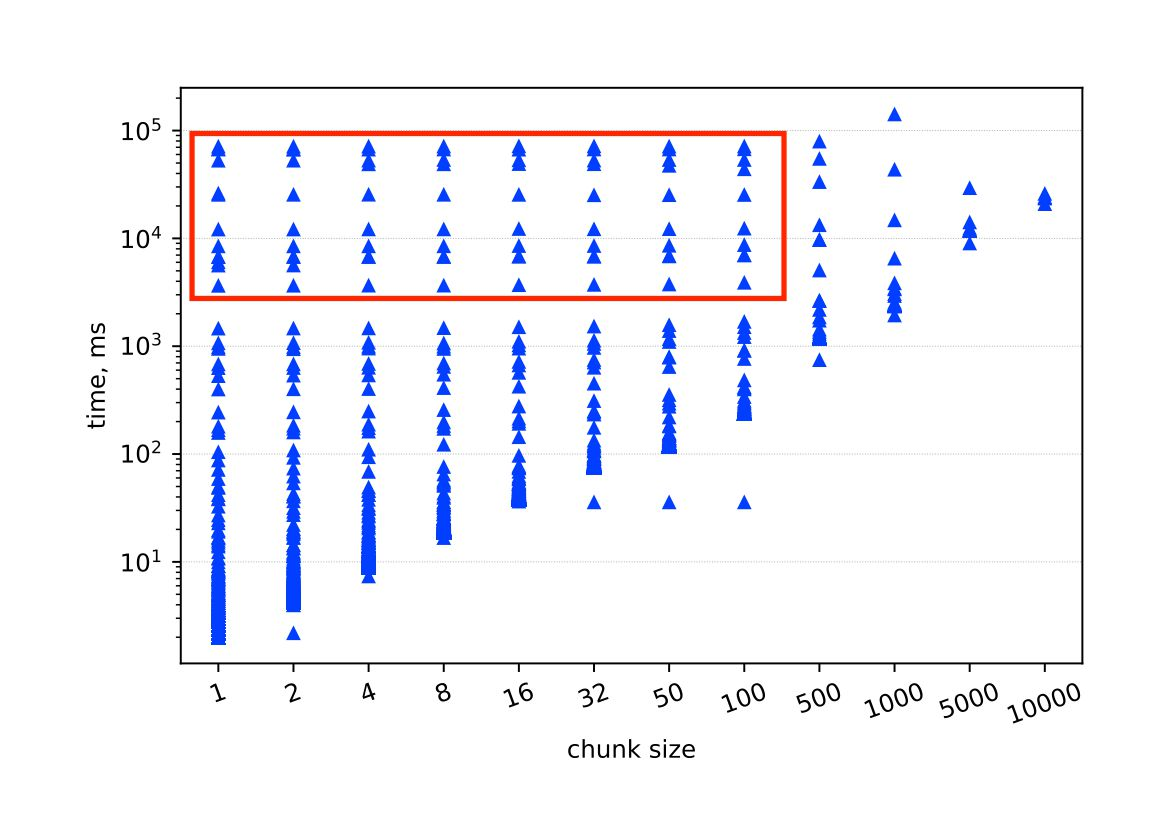
\includegraphics[width=0.7\textwidth]{Pogozhelskaya/pics/subclass_old.pdf_1.jpg}
\label{fig:arch}
\caption{Grammar $G_2$ and Enzyme}
\end{figure}
\end{frame}
  
    \begin{frame}
  \transwipe[direction=90]
 \frametitle{Modifications}
 \begin{itemize}
     \item The modification of the way to get vertices from Neo4j graph database
     \item The optimization of transition between vertices while graph traversal
     \item The optimization of procedure for getting edge labels
     \item The change of result data representation
 \end{itemize}
% Neo4j returns the outgoing edges of a vertex as a \textit{Stream}. All GLL internals were changed to prevent early stream forcing
    \begin{figure}[H]
    \begin{subfigure}[b]{0.5\textwidth}
    \centering
    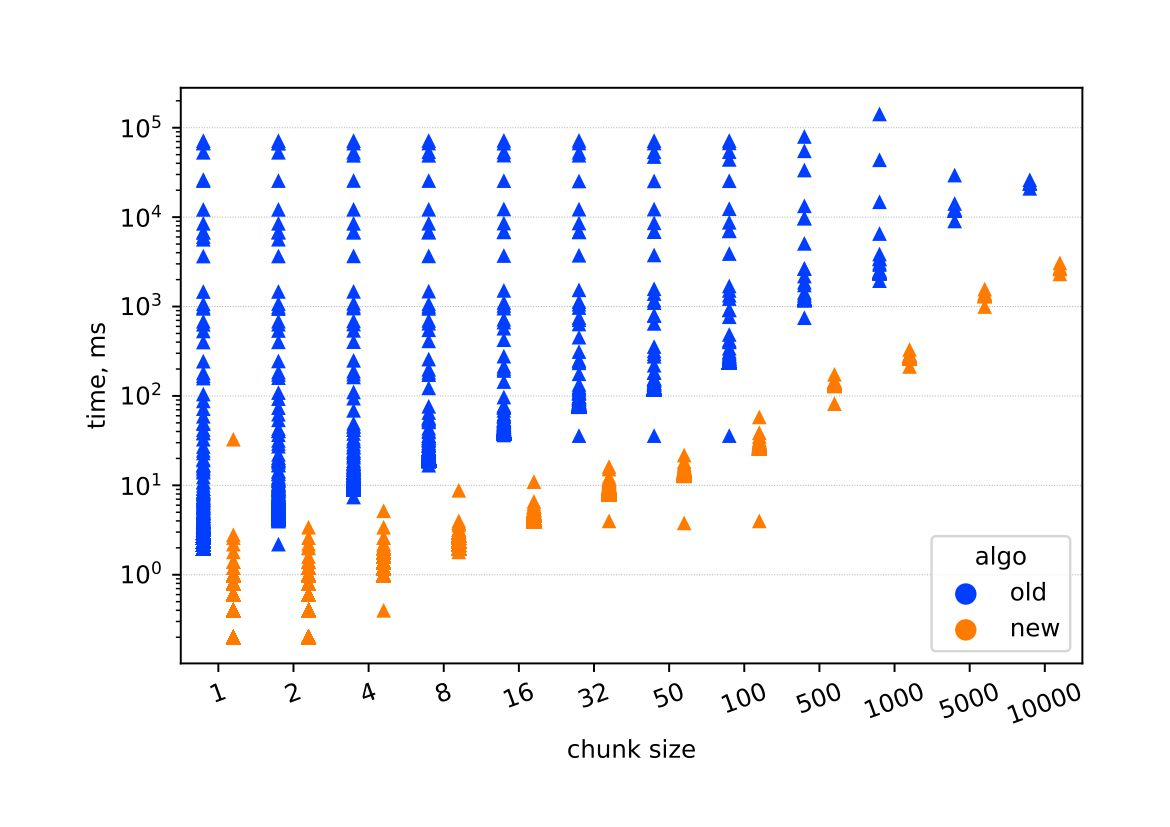
\includegraphics[width=\textwidth]{pics/subclass_old_new.jpg}
    \caption{Query time}
    \label{fig:subim1}
    \end{subfigure}%
    % \hfill
    \begin{subfigure}[b]{0.5\textwidth}
    \centering
    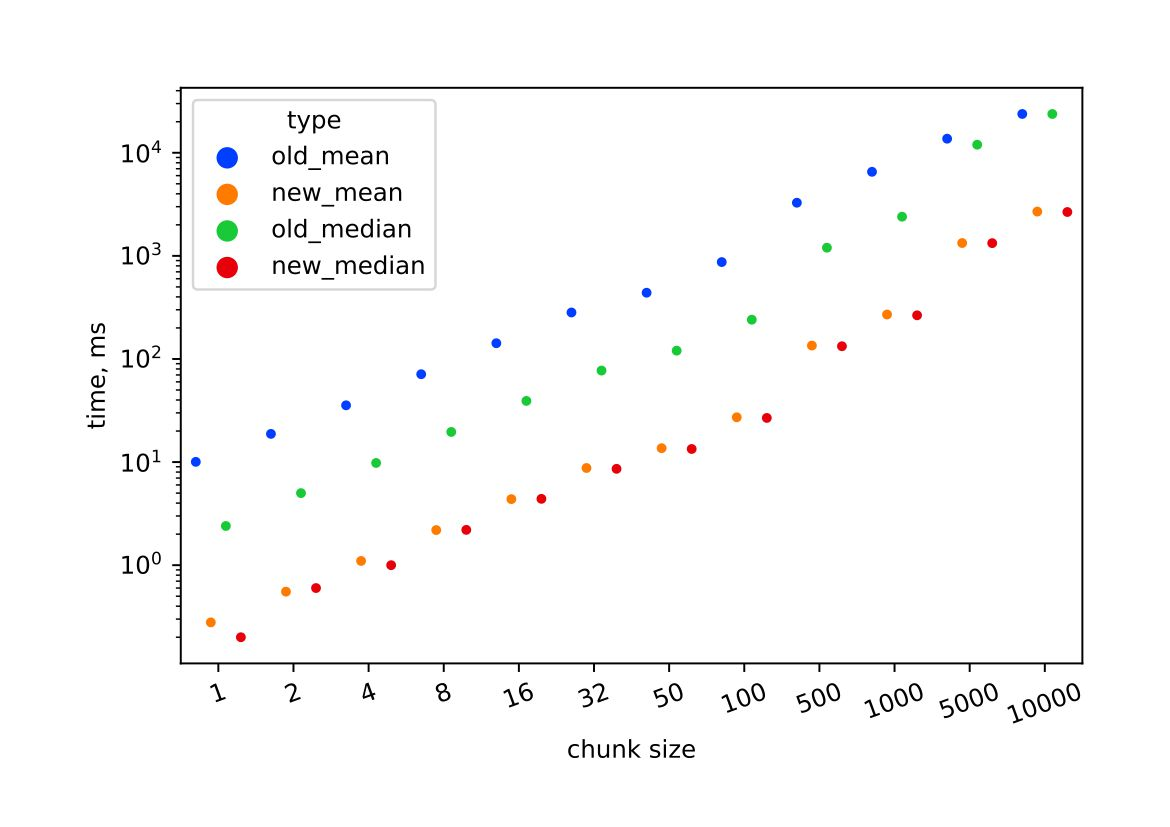
\includegraphics[width=\columnwidth]{Pogozhelskaya/pics/subclass_old_new_m.jpg}
    \caption{Median and mean time}
    \label{fig:subim2}
    \end{subfigure}
    \caption{Grammar $G_2$ and Enzyme}
    \label{old_new2}
\end{figure}
  \end{frame}
  
%   \begin{frame}
%   \transwipe[direction=90]
%  \frametitle{The algorithm improvements performed}
%  \textbf{Performance}
%  \begin{itemize}
%      \item The modification of the way to get vertices from Neo4j graph database
%      \item The optimization of transition between vertices while graph traversal
%      \item The optimization of procedure for getting edge labels
%      \item The change of result data representation
%  \end{itemize}
%   \textbf{Reachability}
%   \begin{itemize}
%       \item The implementation of GLL-based CFPQ algorithm was extended with ability to solve the reachability CFPQ problem
%   \end{itemize}
%  \end{frame}
 
 
  \begin{frame}
   \transwipe[direction=90]
 \frametitle{Extension to solve the reachability problem}
 The ability to switch between the SPPF construction and reachability facts calculation was provided
 \begin{figure}[ht]
    \centering
    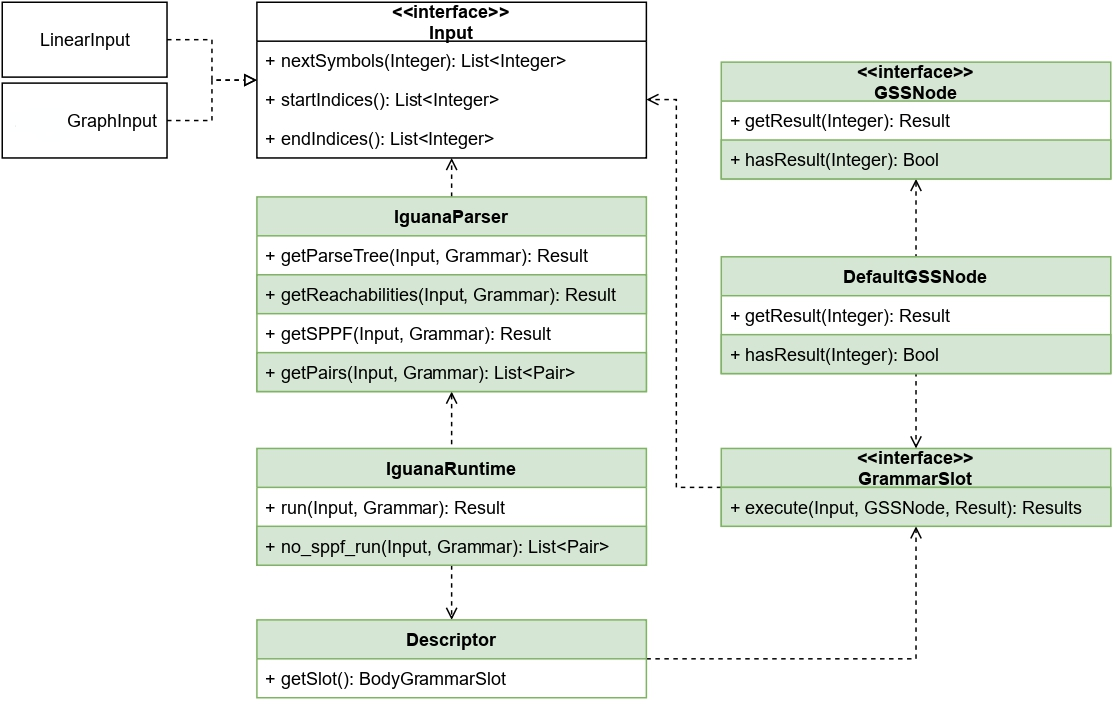
\includegraphics[width=0.8\textwidth]{pics/sppf_arch.jpg}
    \caption{Architecture of the proposed solution}
    \label{fig:solution_architecture}
\end{figure}
  \end{frame}
  
  
  \begin{frame}
\transwipe[direction=90]
 \frametitle{Experimental study setup}
%  \textbf{Scenarios}
%  \begin{itemize}
%      \item Multiple-source all paths after modifications
%      \item All-pairs reachability
%      \item Single-source reachability
%      \item Single-source all-paths
%  \end{itemize}
 \textbf{Data}
 \begin{itemize}
     \item \textbf{RDF Graphs}
     \begin{itemize}
         \item \textit{Grammars}
  \begin{align}
\begin{split}
\label{eqn:g_1}
S \to & \overline{\textit{subClassOf}} \ \ S \ \textit{subClassOf} \mid \overline{\textit{type}} \ \ S \ \textit{type}\\   & \mid \overline{\textit{subClassOf}} \ \ \textit{subClassOf} \mid \overline{\textit{type}} \ \textit{type}
\end{split}
 \tag{$G_1$}
\end{align}

\begin{align}
\label{eqn:g_2}
S \to \overline{\textit{subClassOf}} \ \ S \ \textit{subClassOf} \mid \textit{subClassOf}
 \tag{$G_2$}
\end{align}
\begin{align}
\begin{split}
\label{eqn:geo}
S \to & \textit{broaderTransitive} \ \  S \ \overline{\textit{broaderTransitive}} \\
      & \mid \textit{broaderTransitive} \ \  \overline{\textit{broaderTransitive}}
\end{split}
 \tag{$Geo$}
\end{align}
     \end{itemize}
     \item \textbf{Program analysis graphs}
     \begin{itemize}
         \item 
         \textit{Grammar}
         \begin{align}
\begin{split}
\label{eqn:points_to}
M & \to \overline{d} \ V \ d \\
V & \to (M? \ \overline{a})^* \ M? \ (a \ M?)^* 
\end{split}
 \tag{$PointsTo$}
\end{align}
     \end{itemize}
  \end{itemize}
 \end{frame}
  
%     \begin{frame}
%   \transwipe[direction=90]
%  \frametitle{Experiments after modifications}
% Neo4j returns the outgoing edges of a vertex as a \textit{Stream}. All GLL internals were changed to prevent early stream forcing
%     \begin{figure}[H]
%     \begin{subfigure}[b]{0.5\textwidth}
%     \centering
%     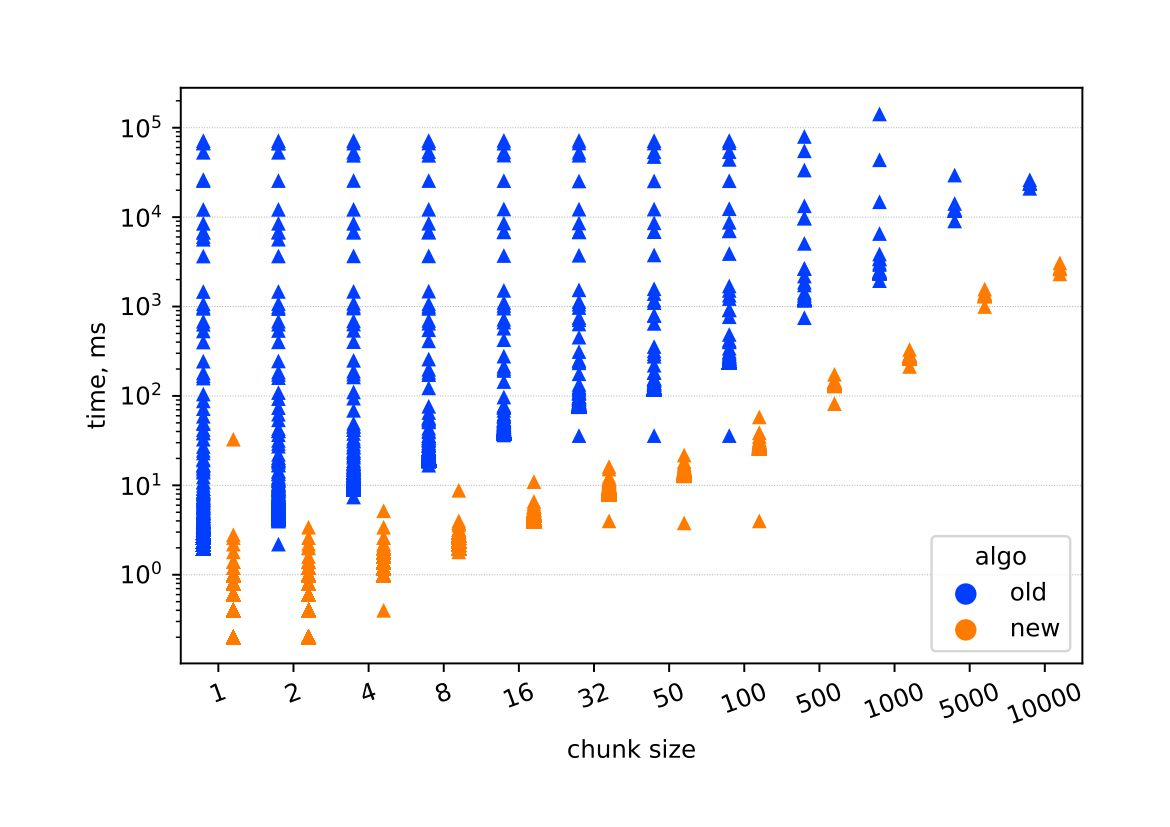
\includegraphics[width=\textwidth]{pics/subclass_old_new.jpg}
%     \caption{Query time}
%     \label{fig:subim1}
%     \end{subfigure}%
%     % \hfill
%     \begin{subfigure}[b]{0.5\textwidth}
%     \centering
%     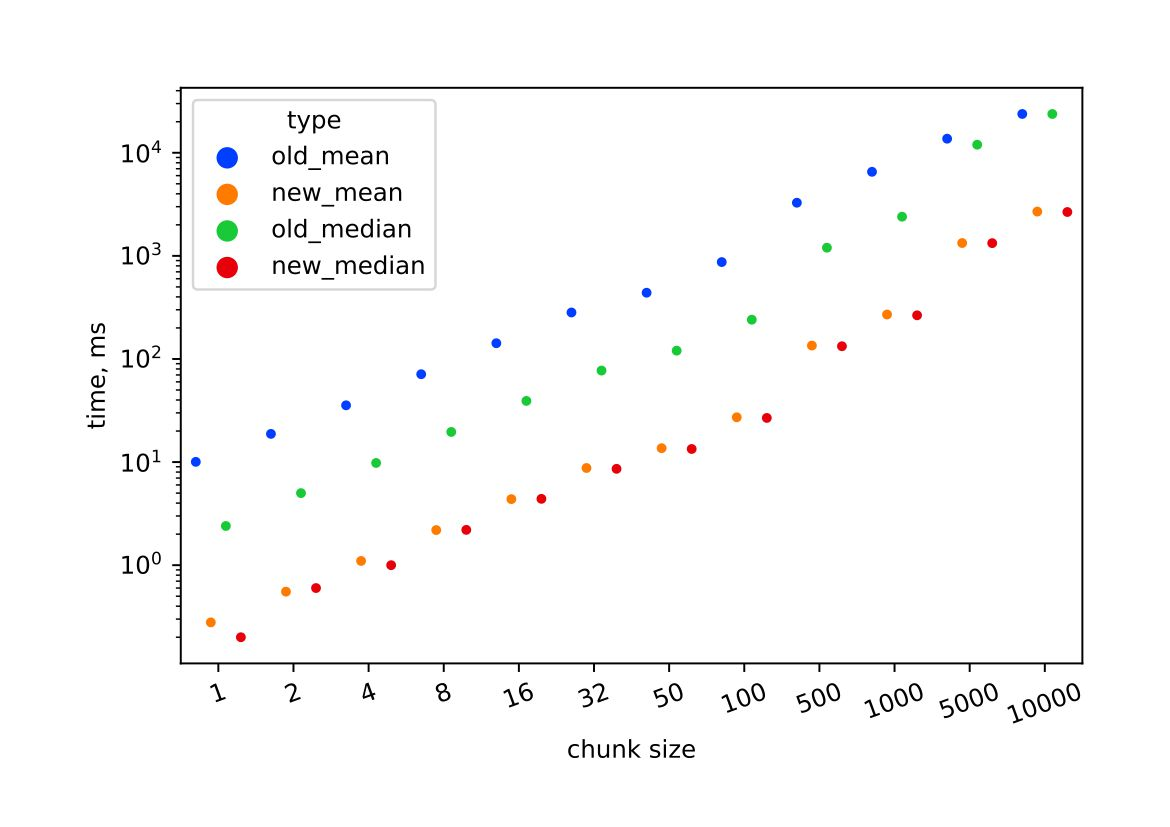
\includegraphics[width=\columnwidth]{Pogozhelskaya/pics/subclass_old_new_m.jpg}
%     \caption{Median and mean time}
%     \label{fig:subim2}
%     \end{subfigure}
%     \caption{Grammar $G_2$ and Enzyme}
%     \label{old_new2}
% \end{figure}
%   \end{frame}
  
 \begin{frame}
\transwipe[direction=90]
 \frametitle{All pairs results for graphs related to \textbf{RDF analysis}}
  \begin{figure}[H]
\centering
\alt<2>{ \textbf{Graphs considered} \\ 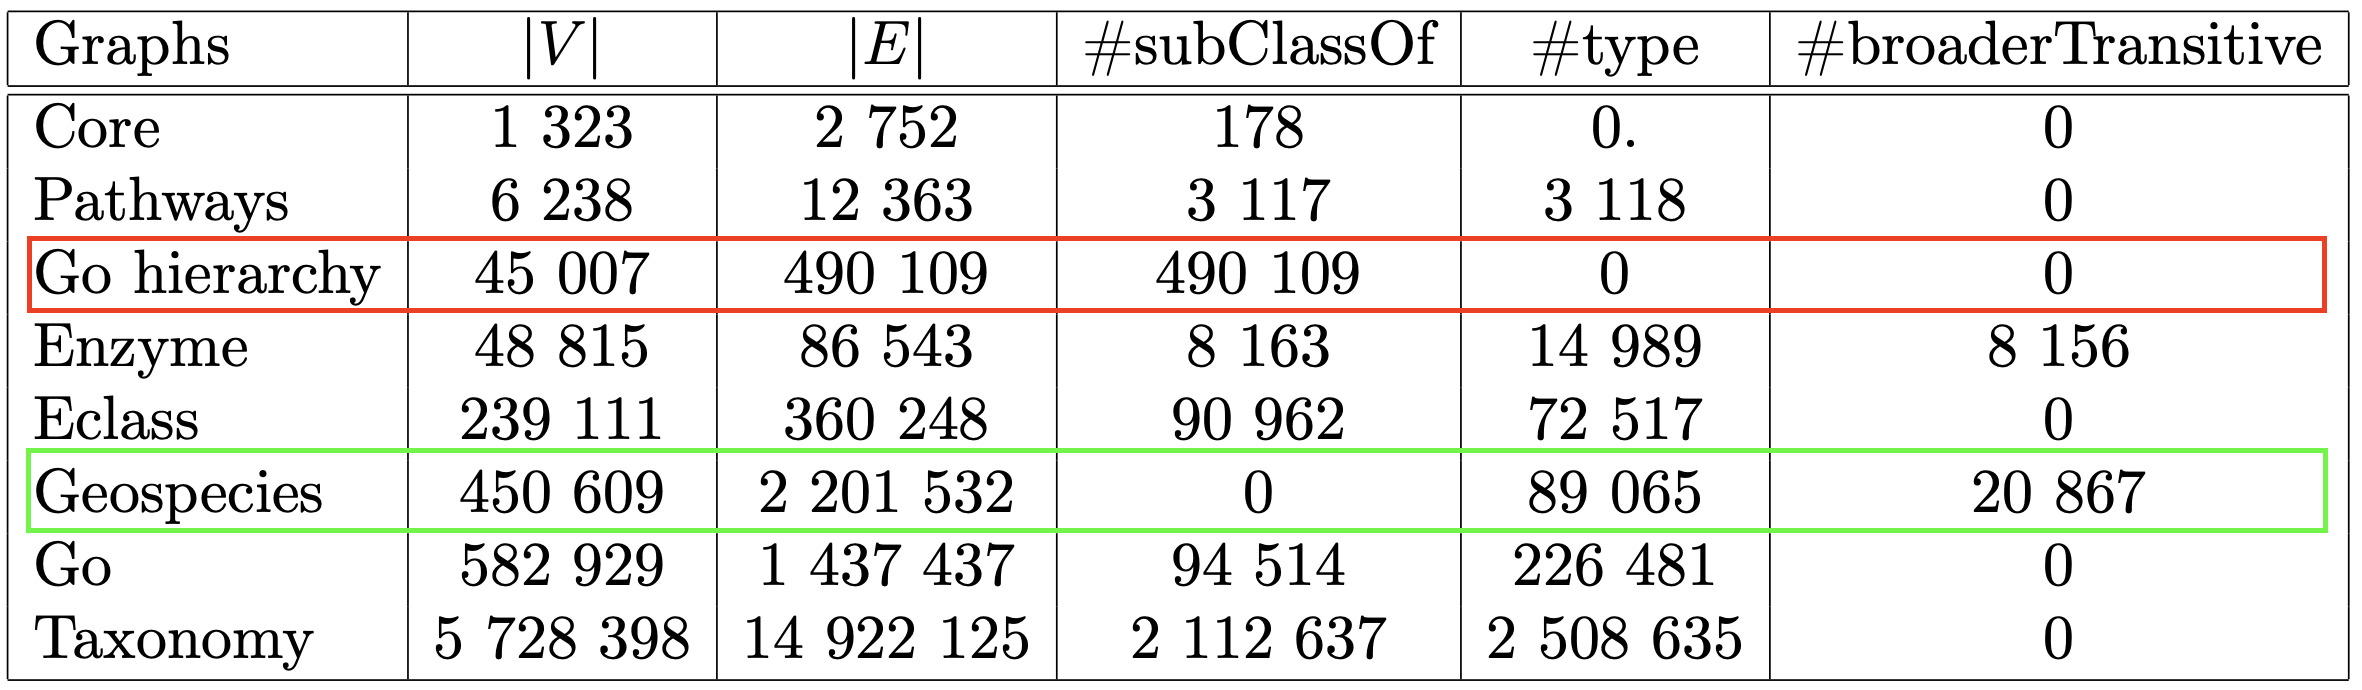
\includegraphics[width=0.73\textwidth]{Pogozhelskaya/pics/nums_rdf_bold.png}}{\textbf{Graphs considered} \\ 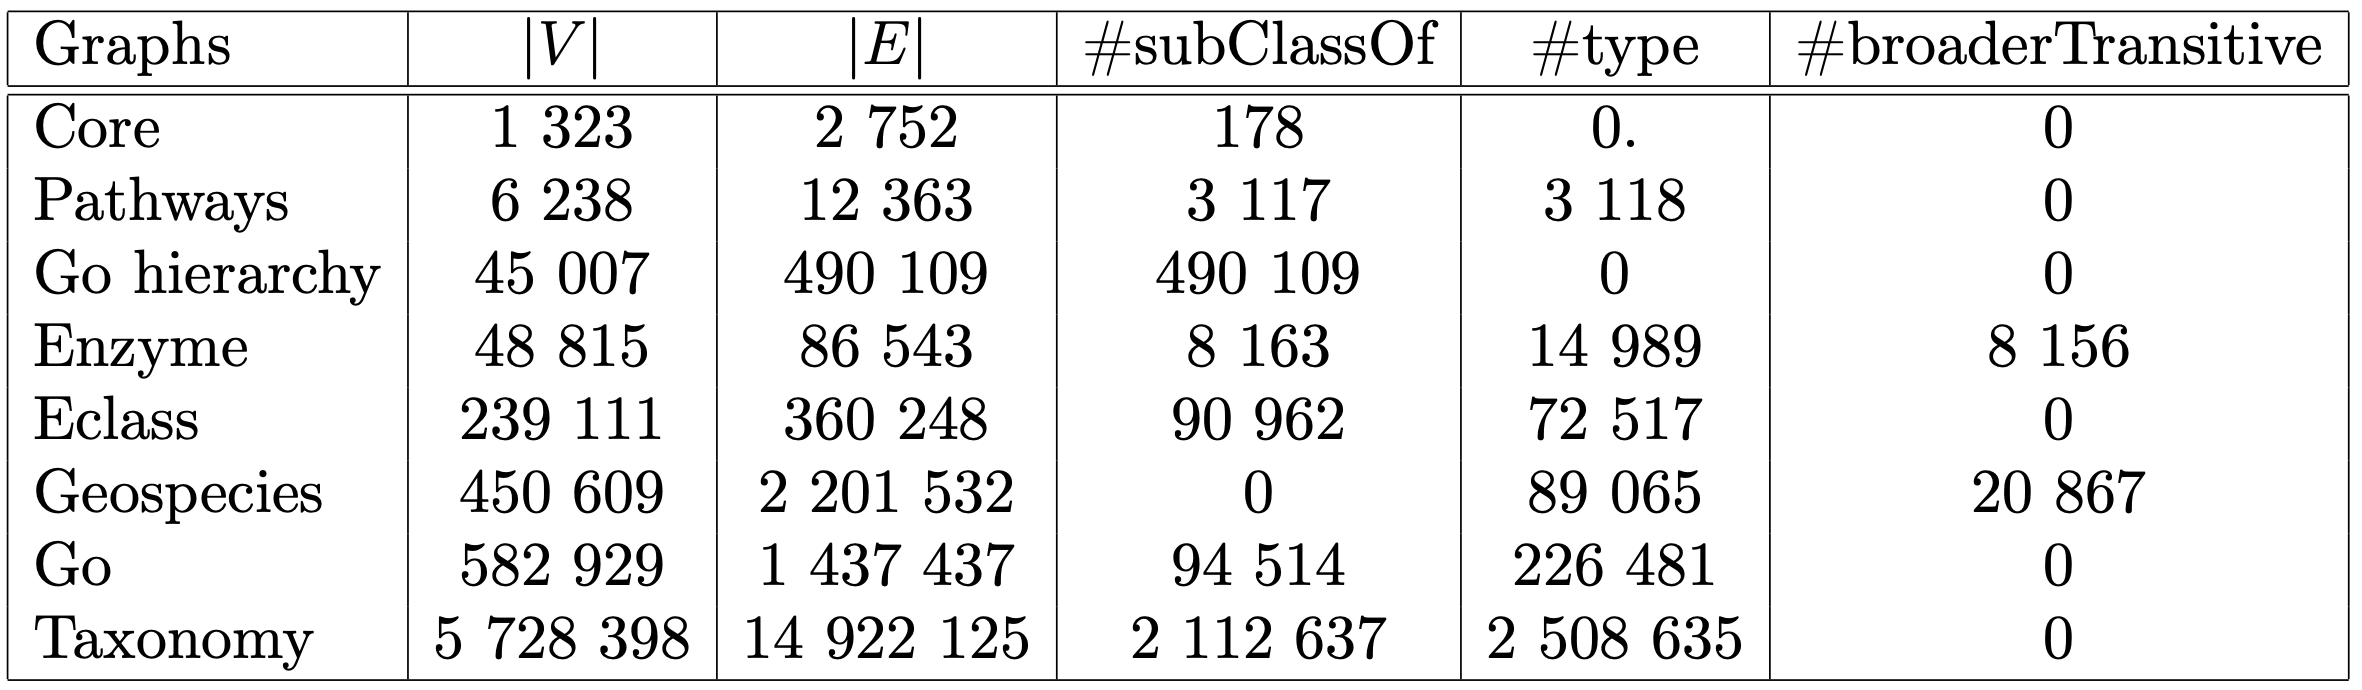
\includegraphics[width=0.73\textwidth]{Pogozhelskaya/pics/nums_rdf.png}}
\label{fig:nums}
\end{figure}

 \begin{figure}[H]
\centering
\alt<2>{\textbf{Results} \\ 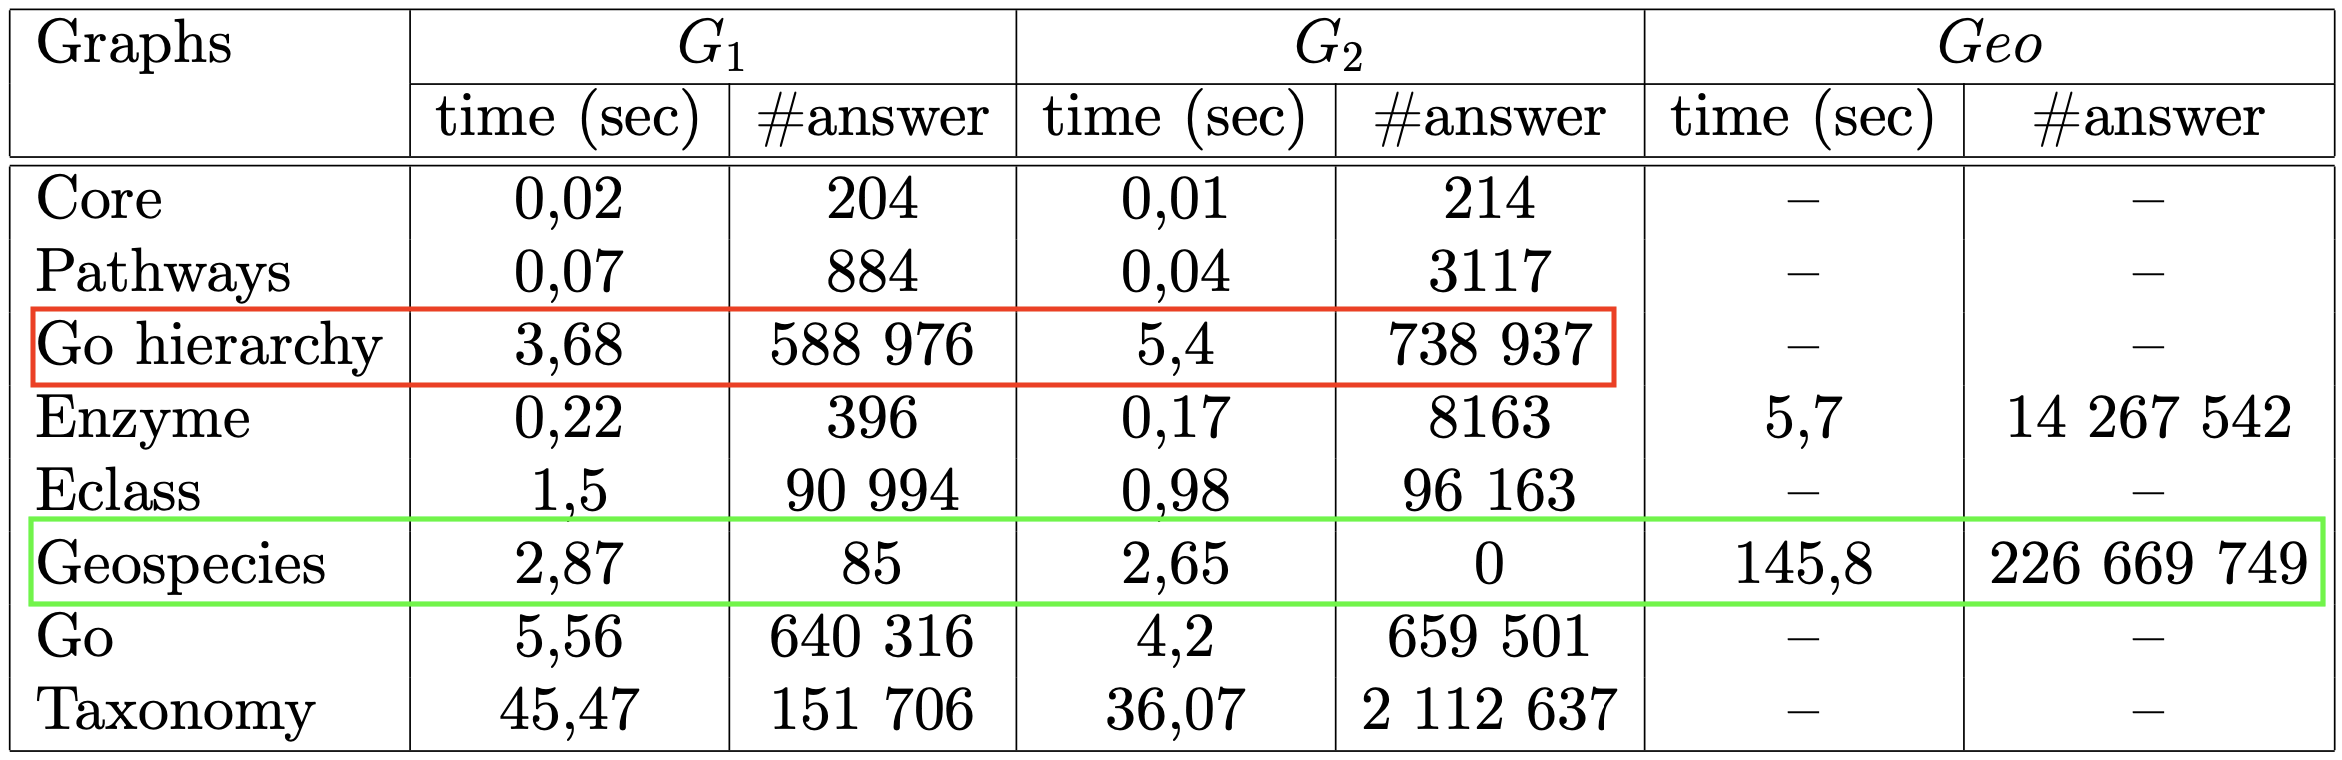
\includegraphics[width=0.73\textwidth]{Pogozhelskaya/pics/res_rdf_bold.png}}{\textbf{Results} \\ 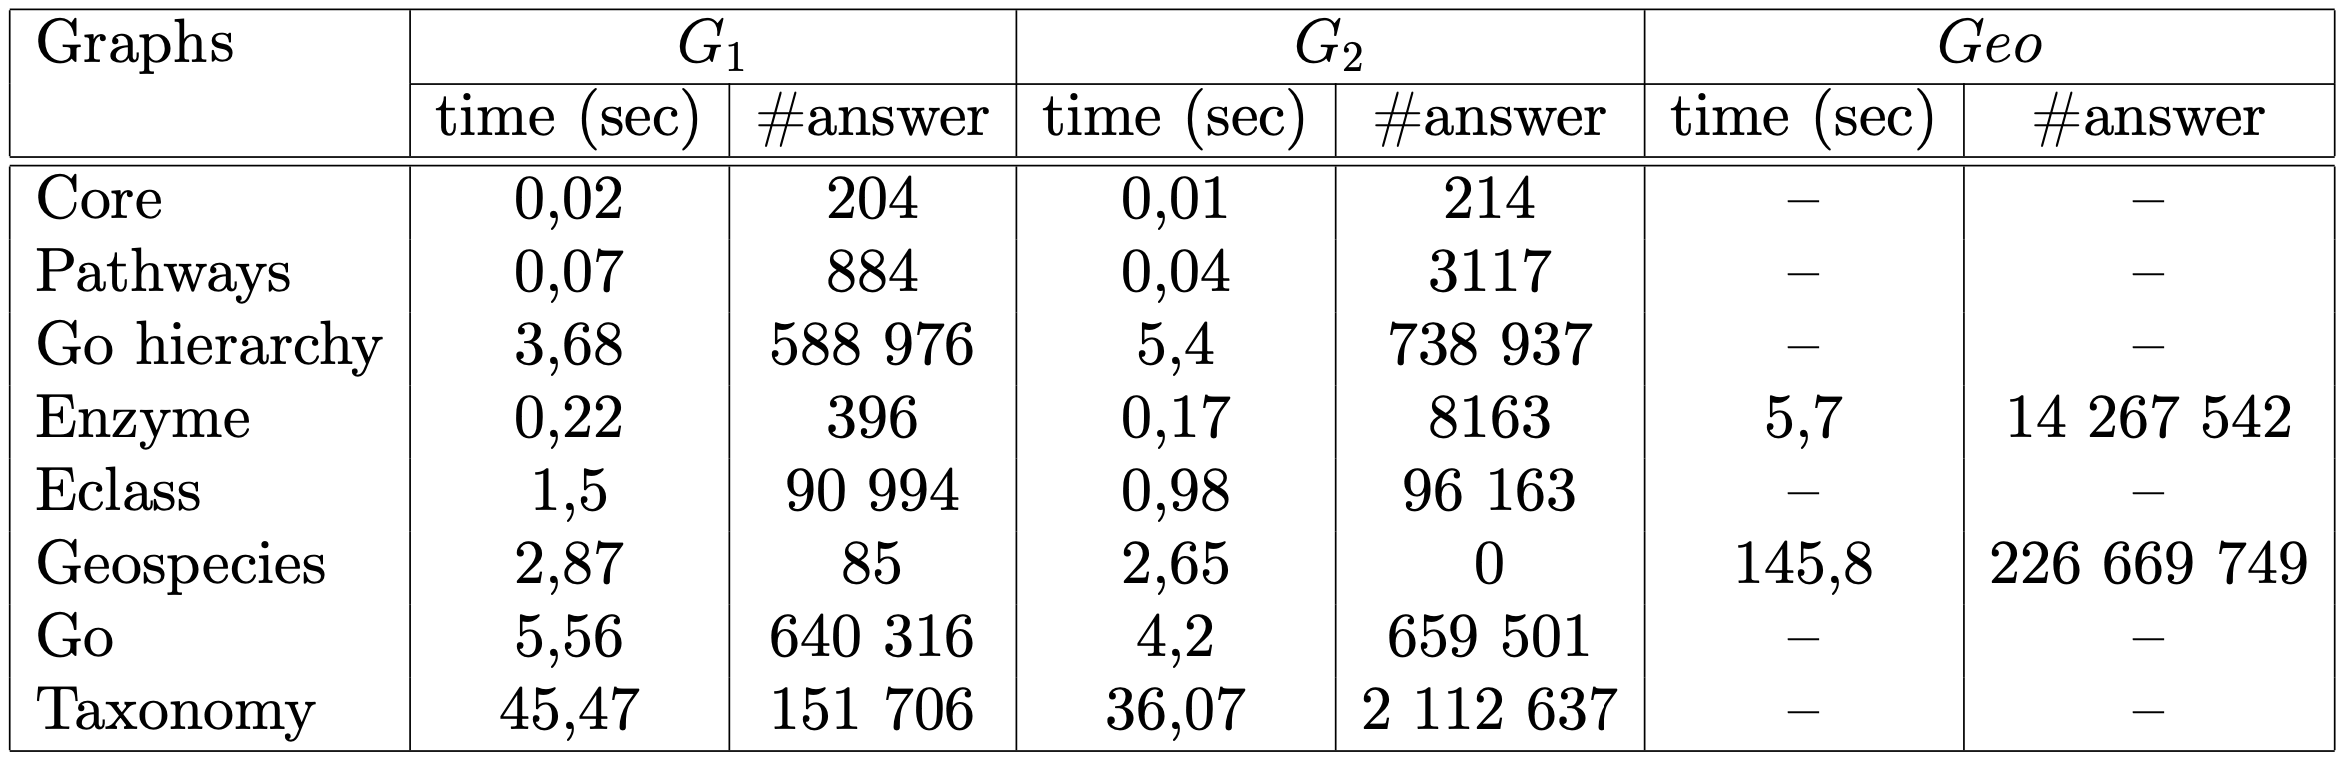
\includegraphics[width=0.73\textwidth]{Pogozhelskaya/pics/res_rdf.png}}
\label{fig:arch}
\end{figure}
\end{frame}

 \begin{frame}
\transwipe[direction=90]
 \frametitle{All pairs results for graphs related to \textbf{static code analysis}}
 
  \begin{figure}[H]
\centering
\alt<2>{\textbf{Graphs considered} \\  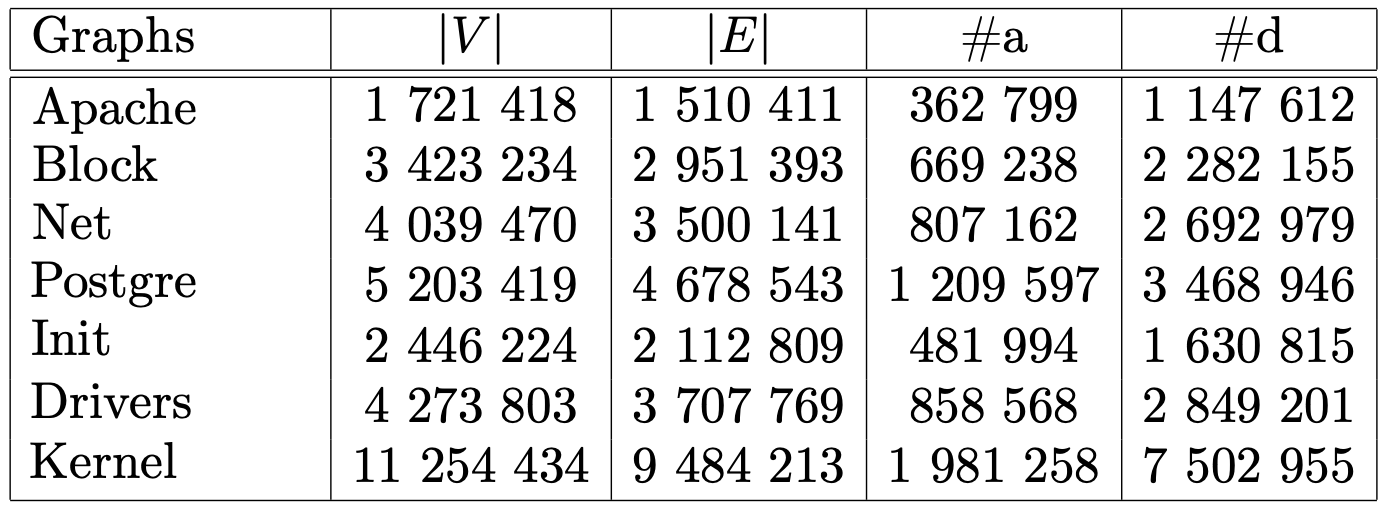
\includegraphics[width=0.73\textwidth]{Pogozhelskaya/pics/stat_res_m.png}}{\textbf{Graphs considered} \\ 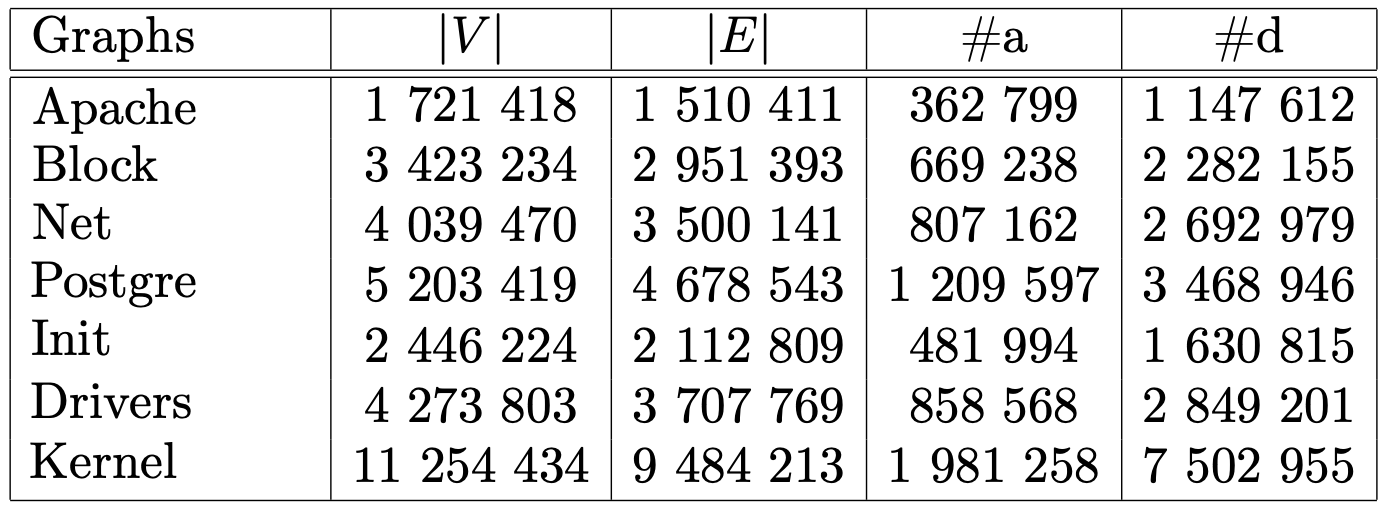
\includegraphics[width=0.73\textwidth]{Pogozhelskaya/pics/stat_res_m.png}}
\label{fig:arch}
\end{figure}

  \begin{figure}[H]
\centering
\alt<2>{\textbf{Results} \\ 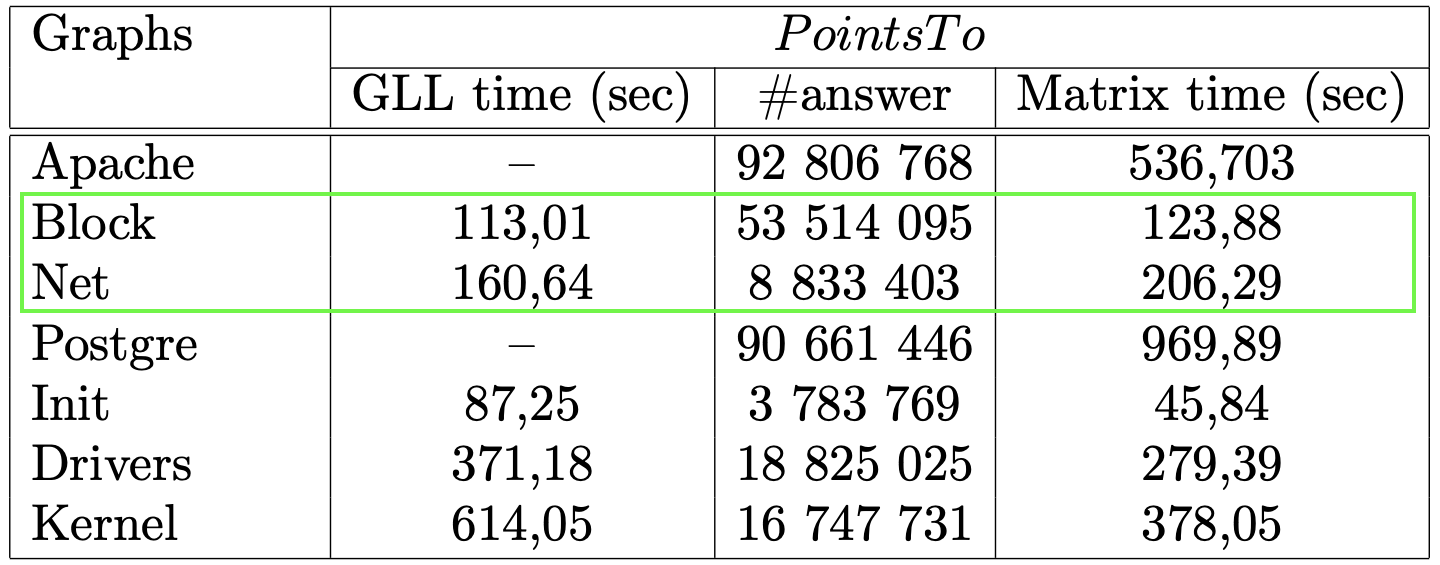
\includegraphics[width=0.73\textwidth]{Pogozhelskaya/pics/stat_nums_bold2.png}}{\textbf{Results} \\ 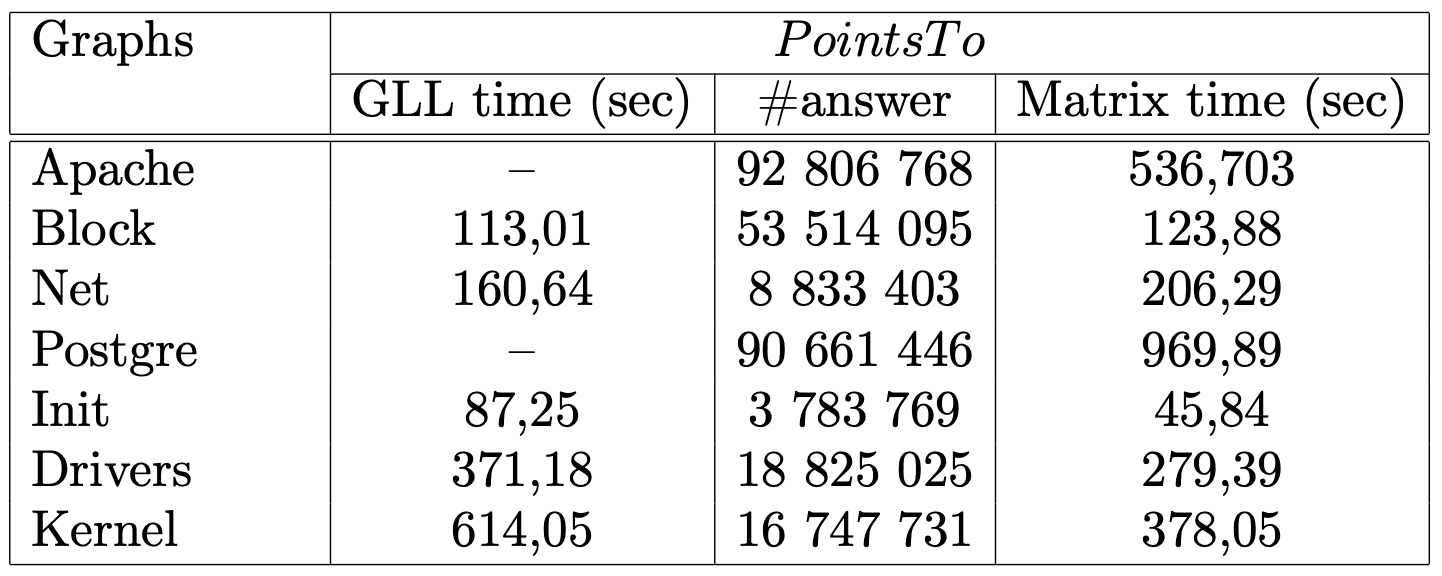
\includegraphics[width=0.73\textwidth]{Pogozhelskaya/pics/stat_nums.png}}
\label{fig:nums}
\end{figure}

\end{frame}


\begin{frame} 
\transwipe[direction=90]
 \frametitle{Single-source results}
 \begin{figure}[H]
\centering
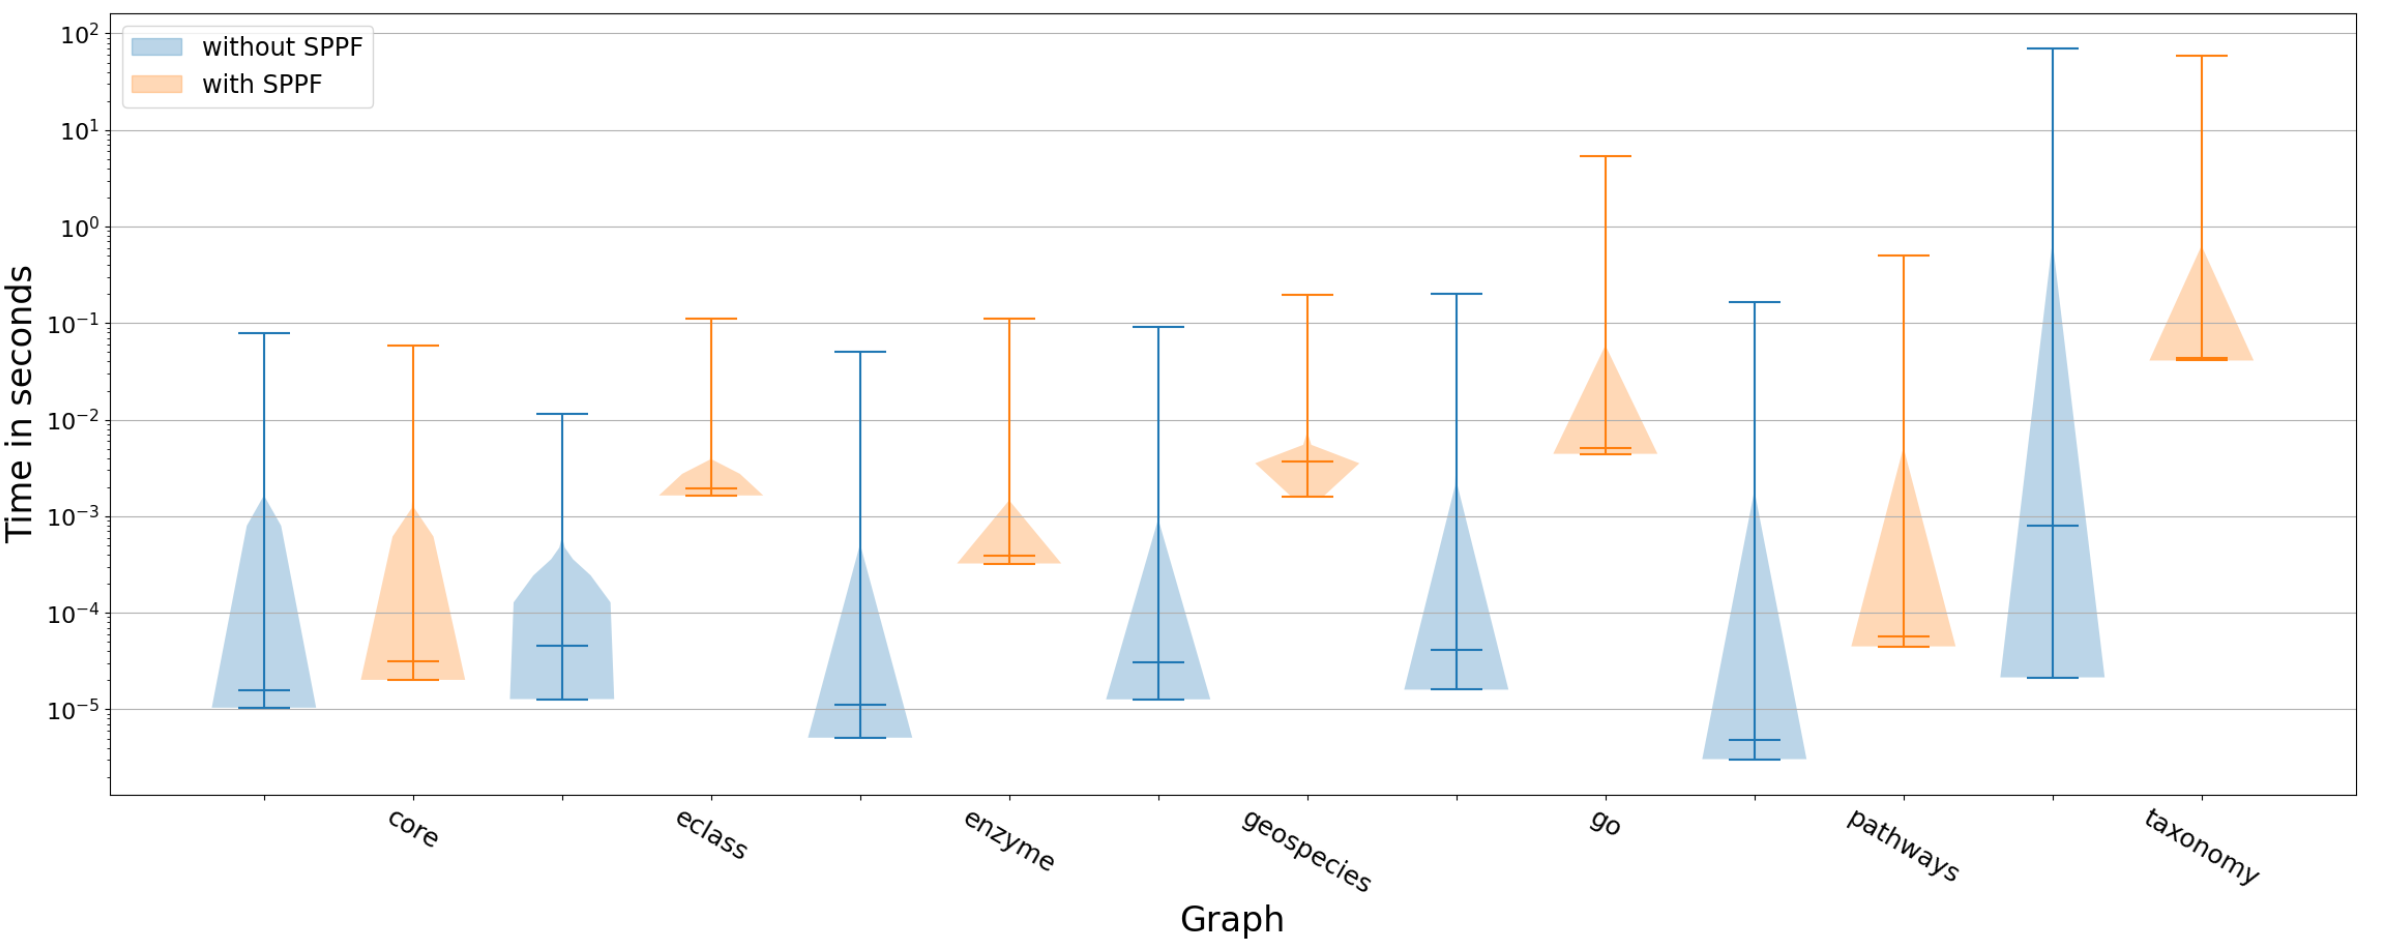
\includegraphics[width=0.82\textwidth]{Pogozhelskaya/pics/ss-rdf.png}
\label{fig:arch}
\end{figure}

\begin{figure}[H]
\centering
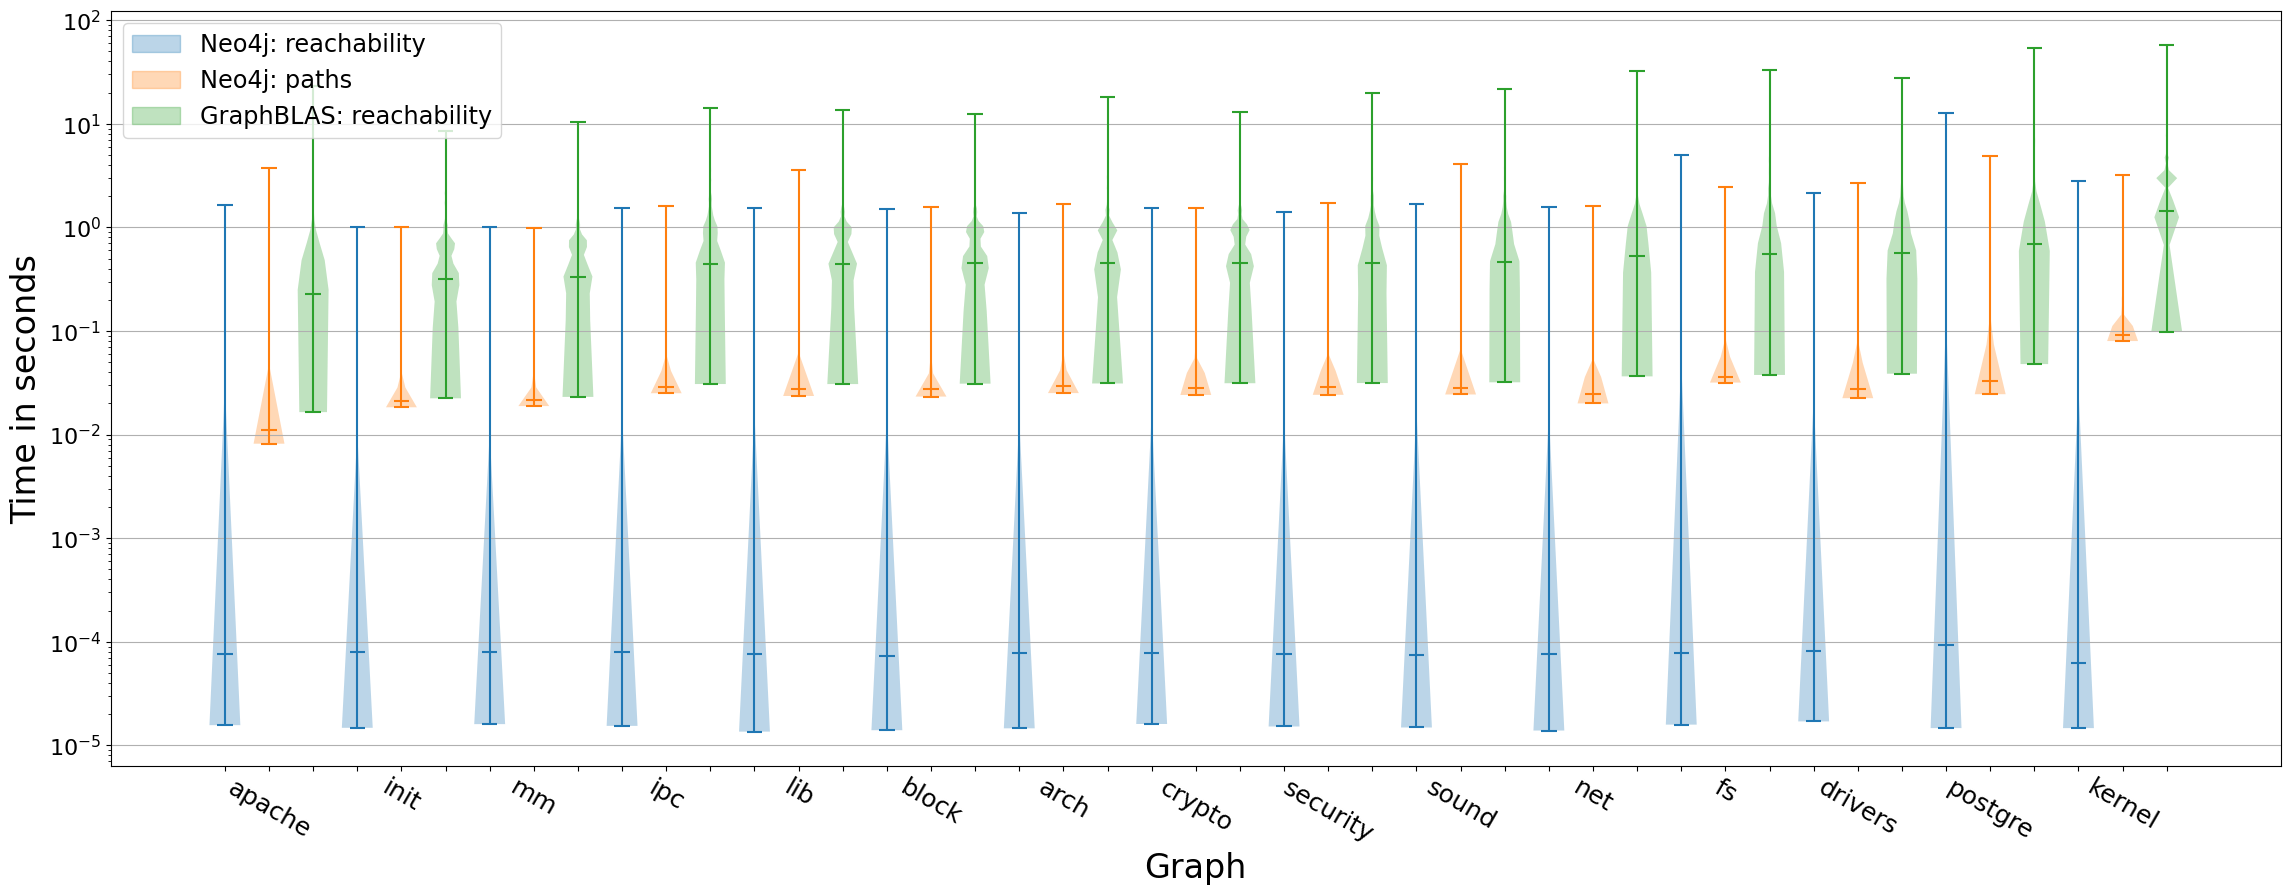
\includegraphics[width=0.82\textwidth]{Pogozhelskaya/pics/stat-m.png}
\label{fig:arch}
\end{figure}

\end{frame}

\begin{frame}
\transwipe[direction=90]
\frametitle{Results}
\begin{itemize}
     \item There were made initial experiments and analysis which confirmed performance problems
    \item The performance problems in the implementation of the GLL-based CFPQ algorithm were eliminated
    \item The implementation of GLL-based CFPQ algorithm was extended with ability to solve the reachability CFPQ problem
    \item The resulting algorithm implementation was evaluated on two sets of real-world graphs: a number of graphs related to RDF analysis and a number of graph related to static code analysis problem for both the \textit{all pairs} and the \textit{multiple sources} scenarios. The evaluation shows that the proposed algorithm is more than 45 times faster than the previous solution for Neo4j
    \end{itemize}
\end{frame}


\end{document}